\chapter{Homework}
\newpage
\section*{Homework 1}
\newpage
\section*{Homework 2}
วันสั่ง: 10 สิงหาคม 2568\\
กำหนดส่ง: เสาร์ที่ 16 สิงหาคม 15:00 น.\\~\\
\noindent โจทย์ ABC Furniture ที่ได้ทำไปในการบ้านที่ 1 แล้ว ได้กำหนดการเชิงเส้นออกมาเป็น
\begin{align*}
    \max \quad & 2000x + 1500y \\
    \texttt{subject to} \quad
    & 4x + 3y \leq 1000 \\
    & 2x + y \leq 800 \\
    & x \geq 0, \quad y \geq 0 
\end{align*}
และมีพื้นที่ของผลเฉลยตามพื้นที่สี่น้ำเงินดังรูปด้านล่าง 
\begin{enumerate}
    \item จงแปลงรูปแบบปัญหาให้อยู่ในรูปแบบมาตรฐานด้วยการเติมตัวแปรส่วนขาด (slack variable)
    \item จงสร้างตาราง simplex ตั้งต้นของกำหนดการเชิงเส้นนี้
    \item และดำเนินการ pivot เพื่อเปลี่ยนตัวแปรฐาน 1 ครั้ง (ระบุตัวแปรฐานขาเข้า กับตัวแปรฐานขาออกด้วย) พร้อมกับอธิบายผลที่ได้เกี่ยวกับการย้ายจุดมุมในรูป
    \item อธิบายว่าจำเป็นต้องทำการดำเนินการ pivot อีกหรือไม่เพราะเหตุใด
    \item แก้โจทย์ปัญหาเดียวกันนี้ด้วยเครื่องมือ Solver ใน Excel
\end{enumerate}
\begin{figure}[h]
    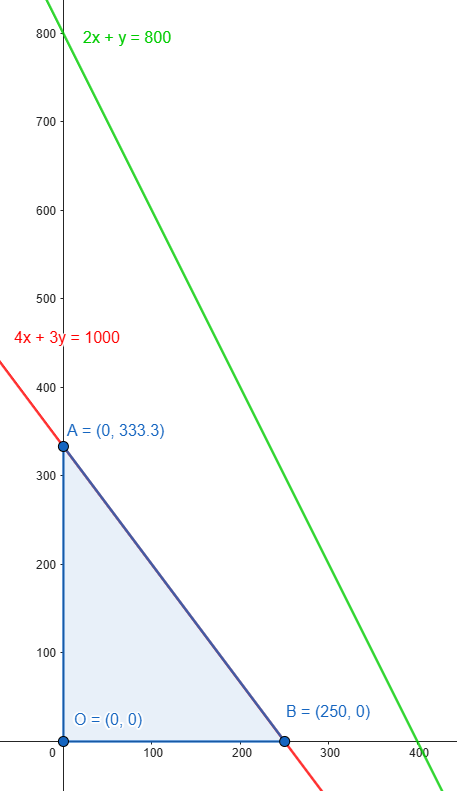
\includegraphics[width=0.37\linewidth]{hw2-1.png}
\end{figure}

\newpage
\section*{Homework 3}
วันสั่ง: 17 สิงหาคม 2568\\
กำหนดส่ง: เสาร์ที่ 23 สิงหาคม 15:00 น.
\subsection*{โจทย์ 1}
\noindent จากโจทย์ ABC Furniture ในเรื่องการกำหนดการเชิงเส้นตามเงื่อนไขที่กำหนดมาให้เราทราบกันมาแล้วว่าตราบใดที่เราสร้างเรากำหนดเงื่อนไขการผลิตโต๊ะ $x$ ตัวและผลิตตู้ $y$ ตัวที่สอดคล้องเงื่อนไขสมการ $4x + 3y = 1000$ ต่างก็จะได้กำไรสูงสุดเช่นกันเสมอ แต่ทั้งนี้สมมติฐานทางธุรกิจของการจะได้กำไรสูงสุดของกำหนดการเชิงเส้นคือต้องสมมติว่าเราจะขายสินค้าที่ผลิตออกมาได้ทั้งหมด ซึ่งอาจจะเป็นไปไม่ได้จริงในสภาวะตลาดที่แตกต่างกัน เพราะบางเวลาโต๊ะก็อาจจะขายได้ดี แต่ในขณะที่บางเวลาตู้ก็อาจจะขายได้ดีกว่า

\textbf{สถานการณ์ทางเลือก:} สำหรับไตรมาสถัดไป ฝ่ายผลิตเสนอ 3 กลยุทธ์ให้ฝ่ายบริหารพิจารณา:

\begin{itemize}
    \item \textbf{กลยุทธ์ A:} ผลิตโต๊ะ 80\% ของการผลิตทั้งหมด
    \item \textbf{กลยุทธ์ B:} ผลิตตู้ 80\% ของการผลิตทั้งหมด
    \item \textbf{กลยุทธ์ C:} ผลิตในอัตราส่วนเท่าๆ กัน
\end{itemize}

\noindent
\textbf{สถานการณ์ตลาด (States of Nature):}  
ฝ่ายการตลาดระบุว่าสถานการณ์ตลาดอาจเป็นไปได้ 3 แบบในไตรมาสหน้า:

\begin{itemize}
    \item \textbf{สถานการณ์ 1 (S1) — โต๊ะบูม:} โต๊ะทำงานขายดีมาก ตู้ขายได้น้อย
    \item \textbf{สถานการณ์ 2 (S2) — ตลาดสมดุล:} สินค้าทั้งสองขายได้ใกล้เคียงกัน
    \item \textbf{สถานการณ์ 3 (S3) — ตู้บูม:} ตู้เอกสารขายดีมาก โต๊ะขายได้น้อย
\end{itemize}

ฝ่ายบริหารต้องการทราบว่า ภายใต้แต่ละกลยุทธ์นั้น ถ้าเกิดสถานการณ์ตลาดแต่ละแบบ จะได้กำไรเท่าไร โดยฝ่ายวิเคราะห์ประเมินกำไร (หน่วย: พันบาท) ดังตาราง:

\begin{center}
\begin{tabular}{|c|c|c|c|}
\hline
\textbf{กลยุทธ์การผลิต} & \textbf{S1: โต๊ะบูม} & \textbf{S2: สมดุล} & \textbf{S3: ตู้บูม} \\
\hline
A (เน้นโต๊ะ) & 422 & 182 & 78 \\
B (เน้นตู้) & 122 & 213 & 378 \\
C (สมดุล) & 284 & 497 & 213 \\
\hline
\end{tabular}
\end{center}

จงตอบคำถามต่อไปนี้
\begin{enumerate}
    \item วิเคราะห์การตัดสินใจภายใต้ความไม่แน่นอนด้วยวิธี maximax
    \item วิเคราะห์การตัดสินใจภายใต้ความไม่แน่นอนด้วยวิธี maximin
    \item ถ้าฝ่ายการตลาดประเมิณมาให้ว่าโอกาสที่จะเกิดตลาดแบบโต๊ะบูม, สมดุล และ ตู้บูมเป็น $25\%, 50\%, 25\%$ ตามลำดับ จงวิเคราะห์การตัดสินใจภายใต้ความเสี่ยงดังกล่าว ด้วยวิธีค่าคาดหวังของกำไร หรือค่าคาดหวังของค่าเสียโอกาสอย่างใดอย่างหนึ่ง
\end{enumerate}

\subsection*{โจทย์ 2}
สถาบันการศึกษาแห่งหนึ่งได้จัดเจ้าหน้าที่เพื่อให้คำปรึกษาวิชาการไว้ 1 คนเพื่อให้คำปรึกษาด้านปัญหาการเรียนแก่นักศึกษา ทว่าได้รับการร้องมาว่าไม่เพียงพอทำให้บางครั้งต้องรอคิวนานจึงกำลังวางแผนจะจ้างเจ้าหน้าที่มาเพิ่มเพราะที่มีอยู่ไม่เพียงพอต่อความต้องการ จึงได้ทำการสำรวจปริมาณการใช้งานในช่วง 1 ชั่วโมง ได้ข้อมูลดังนี้เพื่อจะสุ่มจำลองสถานการณ์โดยใช้เลข 00-99

ข้อมูลการเข้ามารับบริการ\\
\begin{tabular}{|c|c|c|c|c|}
\hline
\textbf{ระยะเวลาที่ห่างกันของการเข้ามา (นาที)} & \textbf{จำนวนนักศึกษา (คน)} & ความน่าจะเป็น & ความน่าจะเป็นสะสม & ช่วงเลขในการสุ่ม \\
\hline 1 & 11 &&&\\
\hline 2 & 29  &&&\\
\hline 3 & 35  &&&\\
\hline 4 & 25  &&&\\
\hline
\end{tabular}

ข้อมูลเวลาในการรับบริการ\\
\begin{tabular}{|c|c|c|c|c|}
\hline
\textbf{เวลาที่ใช้} & \textbf{จำนวนนักศึกษา (คน)} & ความน่าจะเป็น & ความน่าจะเป็นสะสม & ช่วงเลขในการสุ่ม \\
\hline 2 & 15 &&& \\
\hline 3 & 35 &&& \\
\hline 4 & 30 &&& \\
\hline 5 & 20 &&& \\
\hline
\end{tabular}

ได้ทำการจำลองสถานการณ์สำหรับนักศึกษา 10 คน โดยการสุ่มเลขได้ดังตารางด้านล่าง สมมติว่าเริ่มสำรวจตอน 13:00 น.\\
\begin{tabular}{|c|c|c|c|c|c|c|c|c|}
\hline
นิสิต  & เลขสุ่ม   & ระยะห่างเวลา  & เวลาที่ & เวลารอ & เวลาเริ่ม  & เลขสุ่ม &รยะเวลา& เวลาแล้วเสร็จ \\
คนที่ & ระยะห่างเวลา&ระหว่างนักศึกษา& นศ มาถึง &  & ใช้บริการ  & เวลาใช้บริการ &ใช้บริการ& \\
\hline 1 & 53 &&&&&37&& \\
\hline 2 & 74 &&&&&60&& \\
\hline 3 & 05 &&&&&79&& \\
\hline 4 & 71 &&&&&21&& \\
\hline 5 & 06 &&&&&85&& \\
\hline 6 & 49 &&&&&71&& \\
\hline 7 & 11 &&&&&48&& \\
\hline 8 & 13 &&&&&39&& \\
\hline 9 & 62 &&&&&31&& \\
\hline 10 & 69 &&&&&35&& \\
\hline
\end{tabular}

จากตารางการสุ่มที่ได้ จงวิเคราะห์ว่าจำนวนผู้ให้บริการที่มีอยู่เพียงพอหรือไม่

\section*{Homework 4}
วันสั่ง: 24 สิงหาคม 2568\\
กำหนดส่ง: เสาร์ที่ 30 สิงหาคม 15:00 น.

    จากข้อโรงอาหารที่จะได้เมทริกซ์การเปลี่ยนสถานะดังนี้
    \begin{center}
    \begin{tabular}{ll|lll|}
        \cline{3-5}
                                                                     &   & \multicolumn{3}{l|}{เมนูที่ทานเดือนนี้}                   \\ \cline{3-5} 
                                                                     &   & \multicolumn{1}{l|}{A}   & \multicolumn{1}{l|}{B}   & C   \\ \hline
        \multicolumn{1}{|l|}{\multirow{3}{*}{เมนูที่่ทานเดือนถัดไป}} & A & \multicolumn{1}{l|}{0.6} & \multicolumn{1}{l|}{0.6} & 0.2 \\ \cline{2-5} 
        \multicolumn{1}{|l|}{}                                       & B & \multicolumn{1}{l|}{0.3} & \multicolumn{1}{l|}{0.1} & 0.2 \\ \cline{2-5} 
        \multicolumn{1}{|l|}{}                                       & C & \multicolumn{1}{l|}{0.1} & \multicolumn{1}{l|}{0.3} & 0.6 \\ \hline
    \end{tabular}  
    \end{center}
    \begin{enumerate}
        \item จงหาว่าต้องมีอัตราส่วนของคนชอบเมนูอาหารใดเท่าไหร่บ้างถึงจะอยู่ในสภาวะที่ไม่ต้องเปลี่ยนแปลงปริมาณการเก็บวัตถุดิบในเดือนถัดไป (จงหาเวกเตอร์ความน่าจะเป็นที่อยู่ในสถานะคงที่) โดยใช้วิธีการตั้งสมการและแก้ระบบสมการ
        \item ใช้ Excel เพื่อหาเวกเตอร์สถานะคงที่โดยใช้เวกเตอร์ $\begin{pmatrix}
            1 + \text{เลขหลักร้อยของรหัสนักศึกษา}\\
            1 + \text{เลขหลักสิบของรหัสนักศึกษา}\\
            1 + \text{เลขหลักหน่วยของรหัสนักศึกษา}
        \end{pmatrix}$ เป็นเวกเตอร์เริ่มต้น (พิจารณาจำนวนครั้งการคูณกันด้วยตัวเองที่มั่นใจพอว่าเวกเตอร์นิ่งแล้ว) และทำเวกเตอร์สุดท้ายให้อยู่ในรูปเวกเตอร์ความน่าจะเป็น ทำส่งเป็นไฟล์ Excel แนบมาพร้อมกับไฟล์ pdf ของข้อ 1
    \end{enumerate}
    \begin{figure}[h]
        \centering
        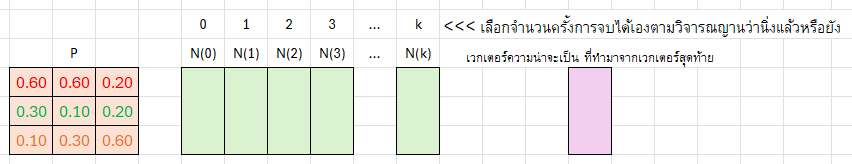
\includegraphics[width=1\linewidth]{Homework4-template.png}
        \caption{ตัวอย่างตาราง Excel (สามารถออกแบบได้ด้วยตัวเอง)}
    \end{figure}
    
\newpage
\section*{Homework 5}
วันสั่ง: 31 สิงหาคม 2568\\
กำหนดส่ง: เสาร์ที่ 6 กันยายน 15:00 น.

\section*{วัตถุประสงค์}
\begin{enumerate}
	\item คำนวณตัวชี้วัดความคลาดเคลื่อน MAE และ RMSE ด้วยมือจากตาราง
	\item เปรียบเทียบความไวต่อ outlier ของ RMSE (ที่ยกกำลังสอง) กับ MAE
	\item ฝึกตีความผลเมื่อมี/ไม่มี outlier ทั้งในชุดฝึกสอนและชุดทดสอบ
\end{enumerate}

\section*{หาตัวแบบ}
\begin{exercise}
	{หาตัวแบบ}{}
	กำหนดชุดข้อมูลมาให้ 6 จุดดังนี้
	\[
	(1,5),\ (2,7),\ (3,9),\ (4,11),\ (5,13),\ \mathbf{(6,50)}
	\]
	โดยที่จุด $(6,50)$ เป็นค่าผิดปกติ (outlier)
	ให้ทำการหาตัวแบบการถดถอยเชิงเส้น 2 อันด้วยการคำนวณด้วยตาราง โดยที่
	\begin{enumerate}
		\item ใช้ข้อมูลครบทั้ง 6 ตัว จะได้ $\hat{y}_{(1)} = \blank{1cm} + \blank{1cm}x$
		\item ใช้แค่ข้อมูล 5 ตัวปกติ จะได้ $\hat{y}_{(2)} = \blank{1cm} + \blank{1cm}x$
	\end{enumerate}
\end{exercise}

\begin{exercise}
	{วัดผลบนชุดข้อมูลที่ใช้สร้างตัวแบบ}{}
	จากตัวแบบที่ได้ในข้อที่ผ่านมา ให้วัดผลด้วย MAE และ RMSE ด้วยชุดข้อมูลที่ใช้
\end{exercise}

\begin{exercise}
	{วัดผลบนชุดข้อมูลใหม่}{}
	จากตัวแบบที่ได้ในข้อที่ผ่านมา ให้วัดผลด้วย MAE และ RMSE ด้วยชุดข้อมูลใหม่ 3 ตัวดังนี้
	\[
	(1.5,6),\ (4.5,12),\ \mathbf{(6.5,55)}
	\]
\end{exercise}

\newpage
\section*{Homework 6}
วันสั่ง: 8 กันยายน 2568\\
กำหนดส่ง: อาทิตย์ที่ 14 กันยายน 21:00 น.

\section*{PART A: ลองคิดกรณีผสมกลยุทธ์ในกรณีที่มีกลยุทธ์แท้}
ตารางค่าผลตอบแทนจากการแข่งขันด้านล่างนี้เป็นตารางของกรณีที่มีกลยุทธ์แท้ กล่าวคือ maximin ของฝ่ายโจมตีมีค่าเท่ากับ minimax การแก้เกมได้ของฝ่ายตั้งรับ
\begin{center}
\begin{tabular}{|c|cc|}
	\hline
	               & \multicolumn{2}{c|}{กลยุทธ์ฝ่ายตรงข้าม}               \\ \hline
	กลยุทธ์ฝ่ายเรา        & \multicolumn{1}{c|}{1}  & \multicolumn{1}{c|}{2}   \\ \hline
	1              & \multicolumn{1}{c|}{4}  & \multicolumn{1}{c|}{3}   \\ \hline
	2              & \multicolumn{1}{c|}{-3} & \multicolumn{1}{c|}{-2}  \\ \hline
\end{tabular}
\end{center}
\textbf{โจทย์:}
\begin{enumerate}
	\item จงหากลยุทธ์แท้ของแต่ละฝ่าย พร้อมทั้งหาค่าของเกม
	\item จงใช้วิธีผสมกลยุทธ์จากฝ่ายเราและวาดแผนภาพแสดงอัตราส่วนของการผสมกลยุทธ์
\end{enumerate}

\section*{PART B: กลยุทธ์ผสม}
ตารางด้านล่างนี้เป็นตารางที่เราได้ดูกันไปในห้องแล้ว และได้ว่าค่าของเกมคือ 36 โดยในห้องเรียนได้พิจารณาการผสมกลยุทธ์ของร้านขาว และการผสมกลยุทธ์แบบสีและแบบผสมของร้านดำไปแล้ว
\begin{center}
	\begin{tabular}{|c|ccc|}
		\hline
		& \multicolumn{3}{c|}{กลยุทธ์ร้านดำ}               \\ \hline
		กลยุทธ์ร้านขาว & \multicolumn{1}{c|}{แบบสี}  & \multicolumn{1}{c|}{แบบขาวดำ}   & \multicolumn{1}{c|}{แบบผสม}\\ \hline
		แบบสี     & \multicolumn{1}{c|}{20}  & \multicolumn{1}{c|}{30}   & \multicolumn{1}{c|}{60}\\ \hline
		แบบขาวดำ   & \multicolumn{1}{c|}{40} & \multicolumn{1}{c|}{45}  & \multicolumn{1}{c|}{30}\\ \hline
	\end{tabular}
\end{center}
ในการบ้านนี้ให้นักศึกษาลองพิจารณาการผสมกลยุทธ์ของแบบสีและแบบขาวดำ (คำเตือน: ต้องพิจารณาแบบ minimax เพราะเป็นตารางผลตอบแทนของร้านขาว)